\documentclass{article}
\usepackage{graphicx}
\usepackage{listings}
\begin{document}

\section{Using Figure 2.2 as a model? illustrate the operation of Insertion-Sort on the array A = (31,41,59,26,41,58).}
\begin{figure}[!htb] 
  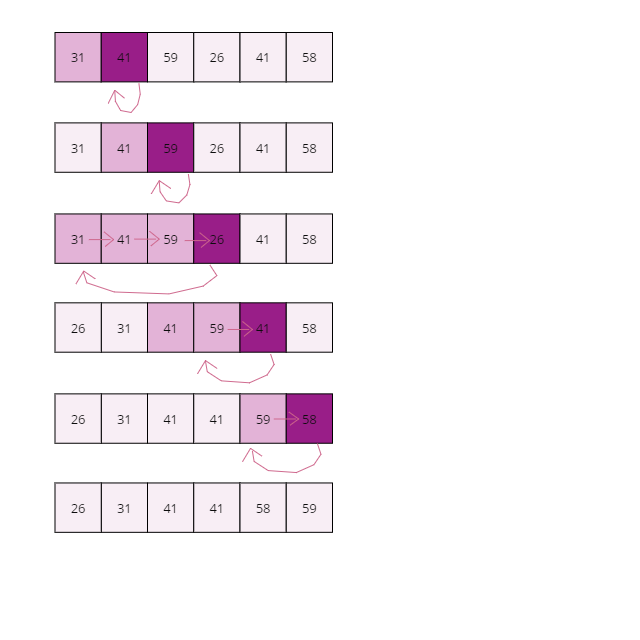
\includegraphics[width=\textwidth]{2_1-1.png}
\end{figure}
 
\section{Rewrite the Insertion-Sort procedure to sort into nonincreasing instead of non-decreasing order.}
\lstinputlisting[language=Python]{2.1-2/nonincreasing-insertion-sort.py}

\section{Consider the searching problem}


Input: A sequence of n numbers = A = (a1,a2,..,an) and a value v.

Output: An index i such that v = A[i] or the special value NIL if v does not appear in A.

Write pseudocode for linear search? which scans through the sequence? looking for v/ Using a loop inveriant, prove that your algorithm is correct. Make sure that your loop invariant fullfills the three necessary properties.
\lstinputlisting[language=Python]{2.1-3/linear-search.py}

\end{document}